% !Mode:: "TeX:UTF-8"
% !TEX program = xelatex

\documentclass[14pt]{Bredelebeamer}
\usepackage{ctex}

\usepackage{multirow}
\usepackage{booktabs}
\usepackage{graphicx}
\usepackage{tikz}
\usepackage{hyperref}
\usepackage{epstopdf}
\usetikzlibrary{arrows,decorations.markings}
\usetikzlibrary{decorations.pathreplacing}
\usetikzlibrary{calc}
 \setbeamerfont{title}{size=\LARGE}
 \setbeamerfont{subtitle}{size=\large}
 \setbeamerfont{institute}{size=\large}
%%%%%%%%%%%%%%%%%%%%%%%%%%%%%%%%%%%%%%%%%%%%%%%%



\title[研究生开题答辩]{基于词表分解优化的循环神经网络语言模型}
\subtitle{Vocabulary Factorized Optimization for \\ Recurrent Neural Network Language Model}
\institute[]{北京航空航天大学中法工程师学院研究生开题答辩}
\author[\href{olivier.shi@buaa.edu.cn}{ \textit{olivier.shi@buaa.edu.cn}}]{是黎彬\\ (\href{mailto:olivier.shi@buaa.edu.cn}{\textit{olivier.shi@buaa.edu.cn}})}
\date{ 2017 年 12 月 20 日}
\subject{开题答辩}

\begin{document}

\begin{frame}
  \titlepage
\end{frame}

\begin{frame}{概览}
  \begin{columns}
    \begin{column}{.5\textwidth}
        \tableofcontents
    \end{column}
    \begin{column}{.5\textwidth}
      \begin{figure}
        \centering
        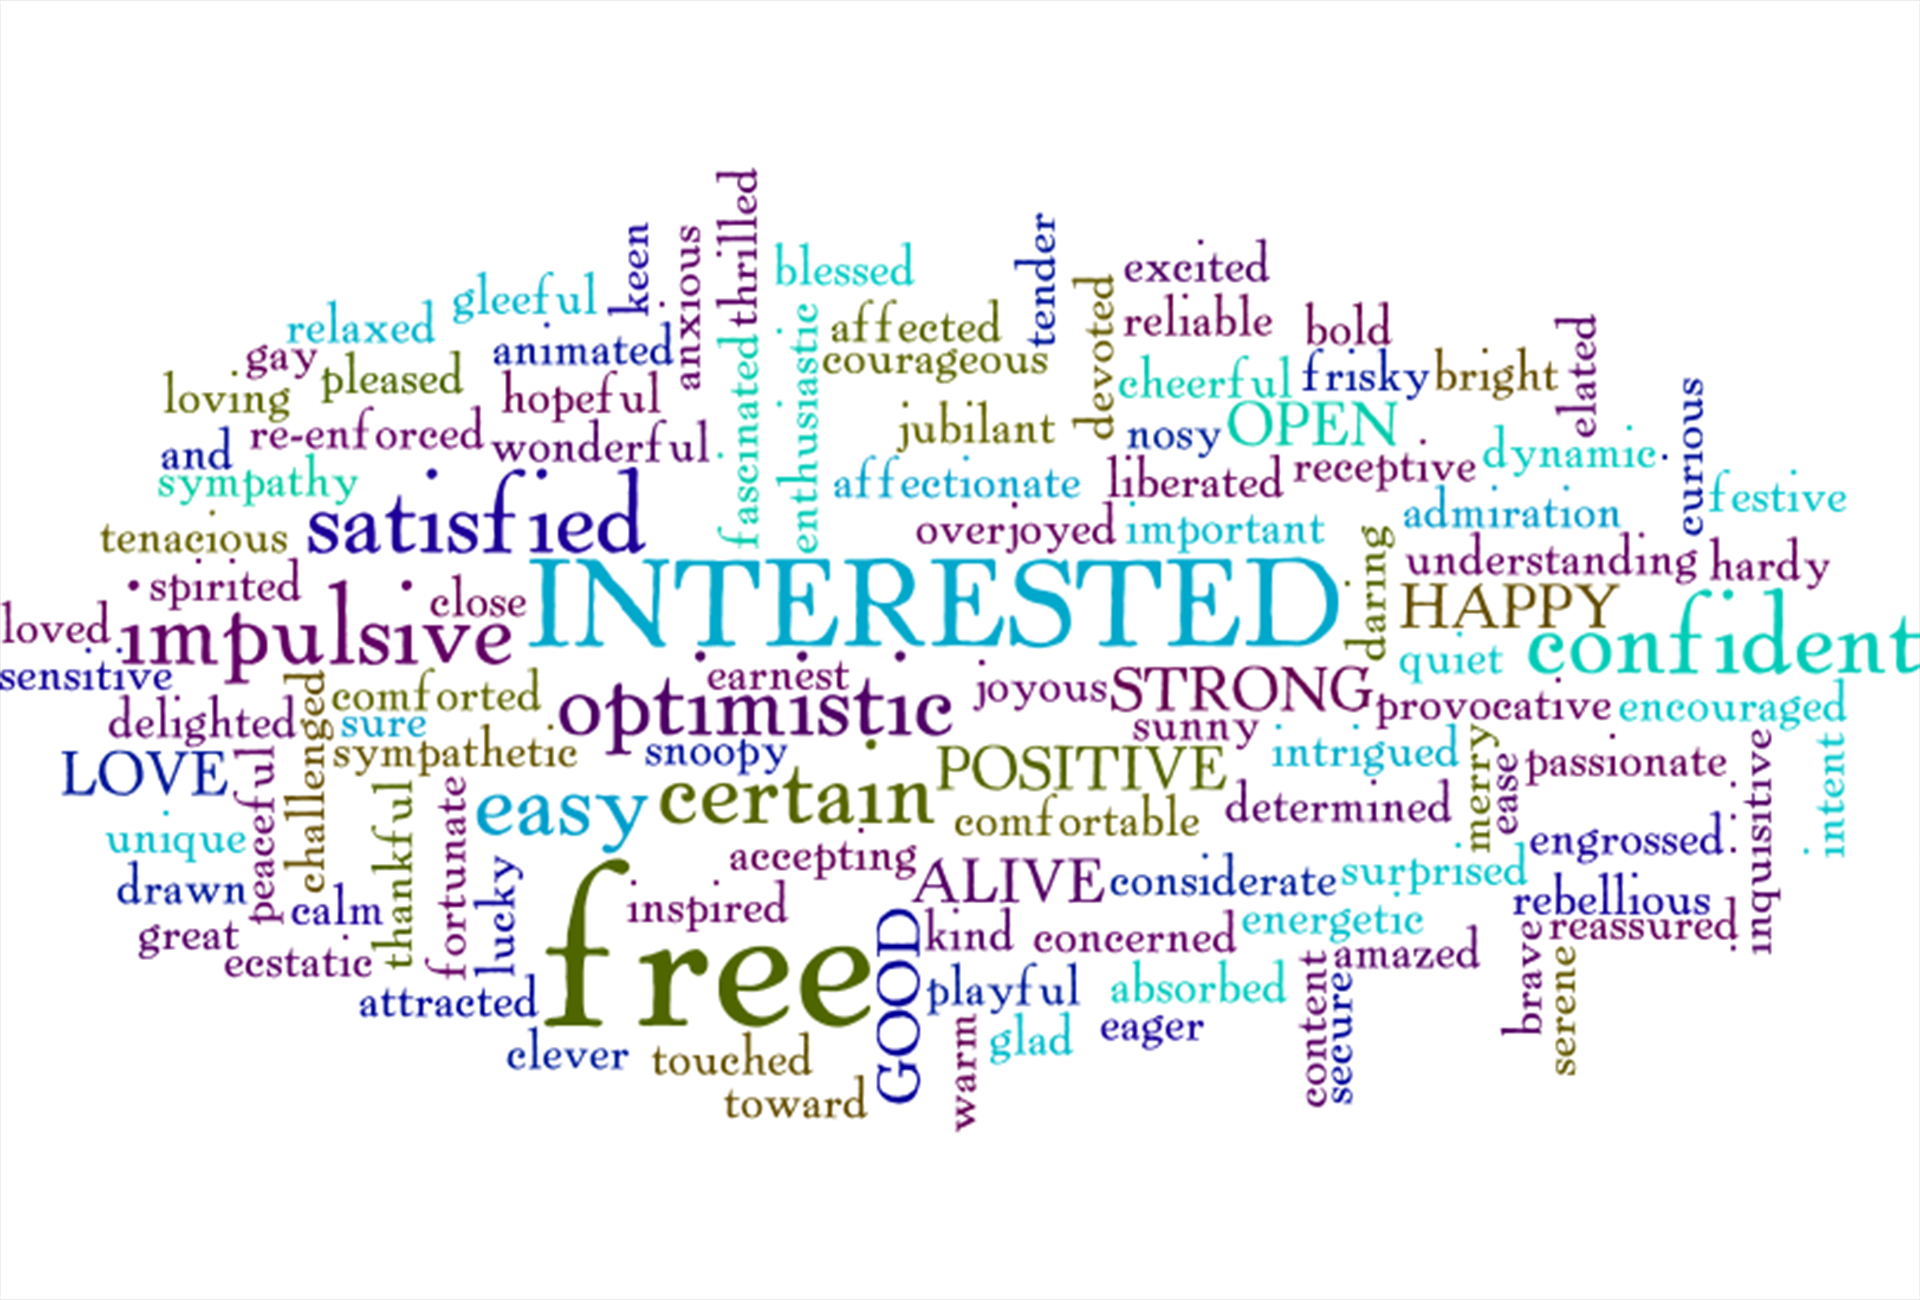
\includegraphics[width=1.\textwidth]{images/word-cloud.png}
      \end{figure}
    \end{column}
  \end{columns}
\end{frame}

\section{论文选题的背景与意义}
\begin{frame}{题目来源}
  论文题目《基于词表分解优化的循环神经网络语言模型》为实验室研究课题。
  \pause
  \begin{alertblock}{语言模型(Language Model)}
    \begin{itemize}
      \item WHAT? 语言模型是学习人类语言的模式,并对一段文本的概率进行估计
      \item WHY? 对信息检索、机器翻译、语音识别等自然语言处理领域中的人物有着重要的作用
      \item HOW? 统计语言模型的作用是为一个长度为T的词序列确定一个联合概率分布$P(w_1;w_2; \cdots ;w_T)$,表示其存在的可能性
    \end{itemize}
  \end{alertblock}
  \pause
  \begin{block}<3->{深度学习与自然语言处理(Deep learning for NLP)}
    \begin{itemize}
      \item 由于人类语言结构的复杂性和数据多样性,传统的方法建模能力有限
      \item 深度学习的提出与发展大大提高了计算机在复杂数据上建模能力,为从结构性较差的数据上学习一定的知识提供模型支撑
    \end{itemize}
  \end{block}
\end{frame}

\section{国内外研究现状及发展动态}
\subsection{循环神经网络语言模型}
\begin{frame}{循环神经网络语言模型}
\begin{columns}
\begin{column}{.7\textwidth}

\end{column}

\begin{column}{.3\textwidth}
\end{column}
\end{columns}
\end{frame}

{\large
语言模型可以对一段文本的概率进行估计,对信息检索、机器翻译、语音识别等任务有着重要的作用。
形式化讲,统计语言模型的作用是为一个长度为m 的字符串确定一个概率分布$P(w_1;w_2;\cdots;w_m)$,表示其存在的可能性,其中$w_1$ 到$w_m$ 依次表示这段文
本中的各个词。一般在实际求解过程中,通常采用下式计算其概率值:
\begin{equation}
\label{equ:lm}
\begin{split}
P(w_1;w_2; \cdots;w_m) &= P(w_1) P(w_2|w_1) P(w_3|w_1;w_2)\cdots P(w_i | w_1;w_2;\cdots;w_{i-1}) \\
&\cdots P(w_m | w_1;w_2;\cdots;w_{m-1})
\end{split}
\end{equation}
在实践中,如果文本的长度较长,公式\ref{equ:lm}右部$\cdots P(w_m | w_1;w_2;\cdots;w_{m-1}) $ 的估算会非常困难。因此,研究者们提出使用一个简化模型:n 元模型(n-gram model)。在n 元模型中估算条件概率时,距离大于等于n 的上文词会被忽略,也就是对上述条件概率做了以下近似:
\begin{equation}
\label{equ:approx}
P(w_i | w_1;w_2;\cdots;w_{i-1})  \approx P(w_i | w_{i-(n-1)};\cdots;w_{i-1})
\end{equation}
}
\end{frame}


\subsection{三大类模型变种}


\begin{frame}{三大类模型变种}
    有非常多研究者在RNNLM基础上做了很多改进,可以大致分成以下3大类:
    \pause
    \begin{block}{基于采样近似方法}
    通过采样技术从词表中选取一部分的词来近似计算RNNLM中的softmax。这一类的方法有重要性采样(Importance Sampling, IS)、噪声对比估计(Noise Contrastive Estimation)以及负采样(Negative Sampling),它们的采样技术不同,但核心的思想都是一样的。
    \end{block}
    \pause
    \begin{block}{基于字符级别建模方法}
    所有英语单纯单词都由26个字母组合构成,Kim基于此发明CharCNN,用字符级别的输入代替原始的词级别的输入,那么这能将词嵌入层的参数从原始的${\mathcal{O}(|\mathcal{V}| \times |\mathcal{D}|)}$ 缩减至${\mathcal{O}(|Char| \times |\mathcal{D}|)}$。
    \end{block}
    \pause
    \begin{block}{基于词表分解预测方法}
    利用词表的结构性和层级性以及条件概率把原来的词的一步预测分解成多步预测问题。这一类的方法有很多,包括基于双层结构Softmax(Class-based Hierarchical Softmax, cHSM)的方法和基于树层级结构Softmax(Tree-based Hierarchical Softmax, tHSM)的方法。
    \end{block}


\end{frame}




\section{主要研究内容}

\subsection{词表过大带来的问题}
\begin{frame}{词表过大带来的问题}
    \begin{columns}
    \begin{column}{.5\textwidth}
        \begin{block}{高计算复杂度\\(High computational complexity)}
        RNNLM中的计算复杂度主要受softmax的影响,其中归一化项${\sum_{w^{'}\in\mathcal{V}} {\exp(z_{w^{'}})}}$ 需要遍历整个词表上对所有词的预测分值进行求和,会带来非常高的计算量并使得模型低效。对于一个大小为${|\mathcal{V}|}$ 的词表,Softmax 的计算复杂度等于${\mathcal{|\mathcal{V}|}}$,那么当词表过大的时候,该模块的计算量就会巨大。

        \end{block}
    \end{column}
    \begin{column}{0.5\textwidth}
        \begin{block}{庞大的模型大小\\(Huge model size)}
        RNNLM中的参数规模受词表大小影响的有嵌入层(Embedding layer)和Softmax层,因为嵌入层要将所有的词都映射到向量空间以及Softmax层要在整个词表空间内去预测。它们分别拥有${\mathcal{O}(|\mathcal{V}| \times |D|)}$和${\mathcal{O}(|\mathcal{V}| \times |H|)}$ 的参数量,其中$|D|$ 和$|H|$ 分别表示嵌入层和隐藏层的维度。

        \end{block}
    \end{column}
    \end{columns}
\end{frame}

\subsection{基于词表分解的语言模型}

\begin{frame}{基于词表分解的语言模型}
    主要包括基于双层结构Softmax(Class-based Hierarchical Softmax, cHSM)的方法和基于树层级结构Softmax(Tree-based Hierarchical Softmax, tHSM)的方法
    \pause
    \begin{block}{cHSM}
    通过条件概率把传统的Softmax预测方法分裂成两个步骤。原来的Softmax 是直接把一个词从词表中预测出来,而cHSM 是先预测这个词属于的类别,然后再在这个类别中预测出具体哪个词,
    \begin{equation}
    \label{eq:cHSM}
	p(w|h)=p(c|h)p(w|c,h)
    \end{equation}

    \end{block}
    \pause
    \begin{block}{tHSM}
    它可以被看作是cHSM 的延伸。tHSM 扩展了cHSM 的思想,把Softmax 层继续分裂,直到把原始的Softmax 分裂成一个树结构(Tree)。所有的词都列在在这棵树的叶子节点(Leaf Node)上,而这棵树的中间节点表示词表的深层次结构。
    \end{block}
\end{frame}



\section{拟采取的技术方案}

\begin{frame}{拟采取的技术方案}
\begin{block}{词表分解优化}
词表具有一定的结构性
\begin{itemize}
\item 调研聚类方法:将一定意义上相似的词聚类,初始化词的二级表示
\item 调研交换算法:初始化的词类关系并不一定符合期望并适合模型的构建,于是要在模型训练过程中动态调整交换词在类中的位置
\end{itemize}
\end{block}
\begin{block}{模型优化}
现有的基于词表分解的语言模型存在一定的问题,比如在预测一个词的类标和类内位置的时候,它们都是依赖同一个隐藏层状态,即根据同一个信息源去预测两个不同空间的量。这在一定程度上可能会减小预测准确率。
\end{block}
\end{frame}


\section{论文研究计划}
\begin{frame}{时间安排}
	\begin{block}{}
\begin{itemize}
  \item 2016年12月 $\sim$ 2017年1月:整理资料,学习深入研究词聚类方法
  \item 2017年2月 $\sim$ 2017年4月:深入研究词表交换算法
  \item 2017年5月 $\sim$ 2017年7月:深入研究基于词表分解的建模方式
  \item 2015年8月 $\sim$ 2015年10月:代码整合,实验验证与完善
  \item 2015年11月 $\sim$ 2015年12月:整理资料和论文撰写
\end{itemize}
    \end{block}
\end{frame}


\begin{frame}{Thanks}
	\centering
    谢谢各位老师和同学!请大家批评指正;

	本次开题报告,文献综述,PPT以及后续研究过程中涉及的代码都会上传至Github:\url{https://github.com/OlivierShi/ecpkn}
	
\end{frame}



\end{document}
